\chapter{Fizika atomsfere}
\subsection{Uvod u meteorologiju}
\textbf{Meteorologija} je nauka koja proučava zakonitosti koje vladaju u Zemljinom vazdušnom omotaču, i sva fizkalna događanja koja se u njemu realizuju. Zajedno sa seizmologijom, koja proučava nemire u Zemljinoj kori, hidrologijom, koja proučava podzemne i površinske vode na Zemlji, te zajedno sa naukom o Zemljinom magnetizmu, meteorologija spada u grupu geofizičkih nauka. Pošto su sve pojave i promjene  koje se zbivaju u atmosferi rezultat fizikalnih zakonitosti, te se one mogu jedino objašnjavati i proučavati valjanom primjenom fizičkih zakona, pa zbog toga meteorologija predrstavlja posebnu oblast  fizike, koju, nazivamo fizikom atmosfere.
	\begin{marginfigure}%
	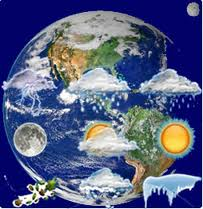
\includegraphics[width=\linewidth]{zemljica}
	\caption{Ilustracija meteorologije i Zemlje}
	\label{fig:zemljica}
	\end{marginfigure} 
Metodi ispitivanja, pa i zaključci koji se iz toga izvode, ne zasnivaju se isključivo na eksperimentu, kakav je slučaj u eksperimentalnoj fizici, gdje se eksperimenti izvode u laboratorijama pod idealiziranim uslovima. U meteorologiji laboratoriju predstavlja atmosfera, gdje se dešavaju promjene zasnovane na zakonima fizike, ali se te promjene izvode pod drugačijim okolnostima nego kad ih izvodmo u laboratorijama, jer se u ovom slučaju radi o laboratoriji gotovo neograničenih dimenzija. Svi procesi, pa čak i oni najkomplikovaniji, koji se odigravaju u atmosferi, mogu se ispravno objasniti jedino primjenom fizikalnih zakona.
Riječ \textbf{meteorologija} vuče svoj korijen od grčkih riječi meteoron i logos, što znači: nauka o onome što je iznad Zemlje, dakle, nauka o atmosferi. Sto se tiče njene starosti, možemo reći da je ova nauka stara gotovo toliko koliko je star i sam čovjek, jer je čovjeka uvijek zanimao taj gasoviti omotač Zemlje bez koga ne bi bilo života. 
	\begin{marginfigure}%
	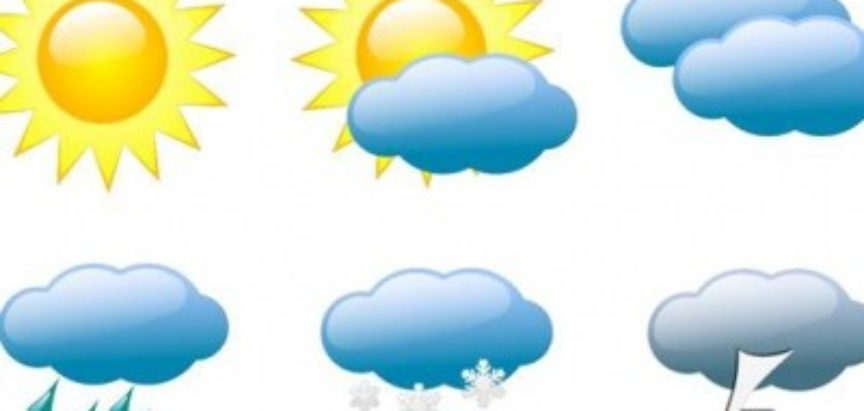
\includegraphics[width=\linewidth]{vremenskaprognoza}
	\caption{Ilustracija prognoze vremena}
	\label{fig:vremenska}
	\end{marginfigure} 
S obzirom na veliku širinu problematike koju danas meteorologija izučava, kao i s obzirom na sve veće zahtjeve koji su se ovoj nauci počeli postavljati, došlo je i u meteorologiji, kao i u ostalim naukama, do podjele na čitav niz naučnih meteoroloških disciplina. Sve brži tempo razvoja privrednih grana, nagli uspon medicinskih i drugih nauka zahtijevao je sve detaljnija proučavanja pojedinih oblasti meteorologije, pa su se te oblasti danas razvile i sve se više razvijaju u posebne naučne i praktične discipline.

Meteorologija se uglavnom može podijeliti na dinamičku meteorologiju, sinoptičku meteorologiju i aerologiju. Dinamička  meteorologija se bavi proučavanjem  kretanja vazdušnih masa, služeći  se fizikalnim dinamičkim i termodinamiokim zakonitostima. Sinoptička meteorologija je u stvari primijenjena meteorologija, i glavni  joj je  zadatak predskazivanje vremena, dok se aerologija bavi proučavanjem procesa u slobodnoj atmosferi. 
\subsection{Pojam i podjela atmosfere}
Prve naučne rasprave o Zemljinoj atmosferi pojavile su se još u starom vijeku, ali je tempo razvoja i napredovanja te naučne misli bio spor, da bi napredovanjem fizike i astronomije to se promijenilo. 
Vazdušni gasoviti omotač koji obavija Zemlju sa svih strana i koji se okreće i pokreće zajedno sa njom u svemiru, zove se atmosfera. Visina atmosfere nije do danas tačno utvrđena, a prema zakonima kinetičke teorije ona i ne može imati jasno definisanu gornju granicu, ali sa druge strane, ta granica bi ipak teorijski morala postojati, i to na onoj visini na kojoj Zemljina teža i centrifugalna sila, koje djeluju na vazdušne čestice, imaju iste vrijednosti. Prema proračunima izvedenim na toj osnovi izlazi da bi se gornja granica atmosfere nalazila na udaljenosti od $5.6$  Zemljinih poluprečnika. 
	\begin{marginfigure}%
		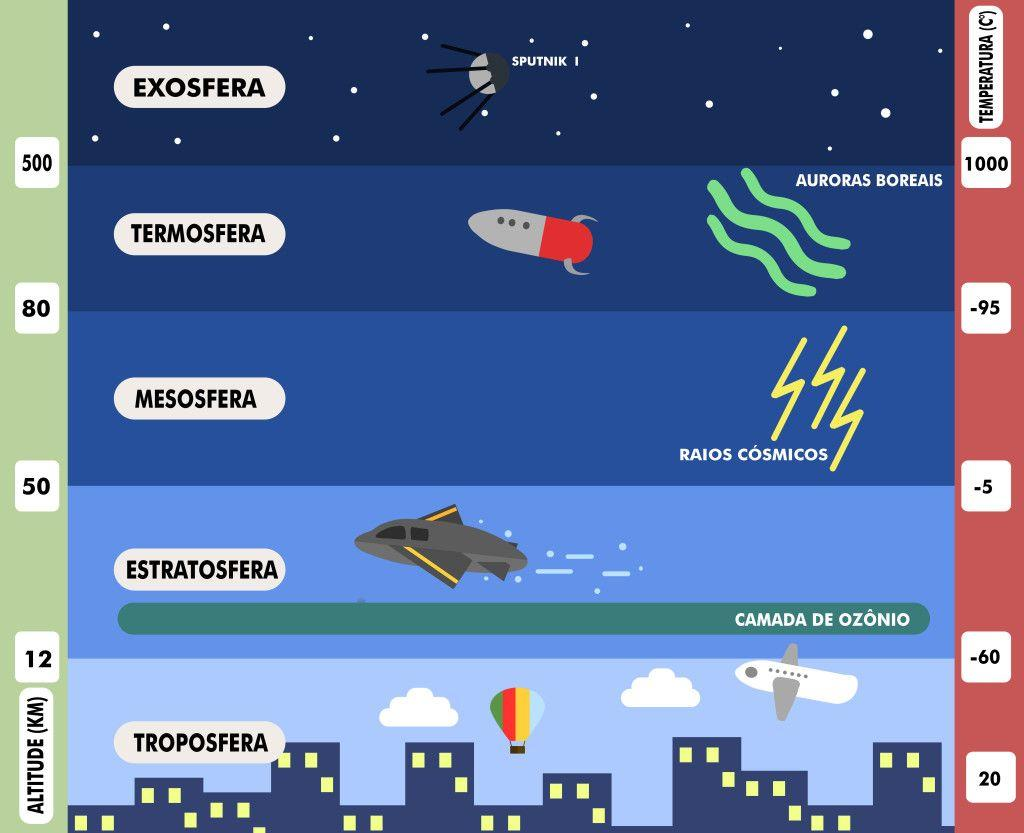
\includegraphics[width=\linewidth]{atmosfera}
		\caption{Podjela atmosfera}
		\label{fig:atmosfera}
	\end{marginfigure}
Tako bi njena visina na ekvatoru iznosila $35711km$, a na polovima 21644km. Najnovija mjerenja vazdušnog pritiska na visini od 200km su pokazala da je vazduh na toj visini toliko razrijeđen da vazdušni pritisak tamo iznosi nešto oko jednog stotog dijela $mm Hg$. Prilikom mjerenja visine na kojoj se pojavljuje polarna svjetlost, ustanovljeno je prisustvo vazduha, prvenstveno azota i ozona, na visinama i od $1000km$, pa i nešto većim. Prema tome, Zemljina atmosfera nije na gornjem dijelu ograničena već ona postepeno prelazi u »atmosferu« međuzvjezdanog prostora koji nigdje nije potpuno prazan. No, visina atmosfere u kojoj je još moguć život čovjeka i velikog broja živih bića sigurno ne prelazi $10km$, jer je ustanovljeno da čovjek veoma teško podnosi visine veće od $6km$.
		\begin{marginfigure}%
		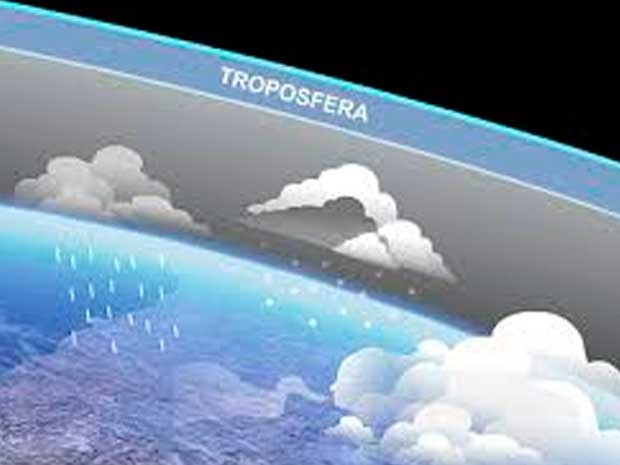
\includegraphics[width=\linewidth]{troposfera}
		\caption{Ilustracija troposfere}
		\label{fig:troposfera}
		\end{marginfigure} 
U odnosu na ponašanje pojedinih meteoroloških elemenata i pojava na raznim visinama atmosfera ima slojevitu strukturu. Sa porastom visine najizraženije ponašanje ima temperatura. Baš po ovom elementu usvojena je šema vertikalne podjele atmosfere na Zasijedanju Međunarodne geodezijske i geofizičke unije 1951. godine. Prema toj šemi atmosfera se dijeli na pet osnovnih sfera ili slojeva, i to: troposferu, stratosferu, mezosferu, termosferu i egzosferu.\\
\textbf{Troposfera} je najniži i najtanji sloj atmosfere. Prostire se od Zemljine površine do 8-10km, odnosno $10-12$ i $16-18km$ iznad polarnih, odnosno umjerenih i tropskih širina. U ovom sloju, iako je najtanji, nalazi se oko $3/4$ mase atmosfere .  U njemu se nalazi skoro cjelokupna količina vodene pare, stvaraju se oblaci i magle, dolazi do pojave padavina u tečnom i čvrstom obliku, razvijaju se grmljavinske nepogode, javljaju se horizontalna i vertikalna kretanja vazduha, turbulencija, mlazna struja i druge meteorološke pojave.\\
Najbitnija osobina troposfere je opadanje temperature sa po¬rastom visine, koje u prošeku iznosi 6.5° na jedan kilometar. Najveći broj aeroloških mjerenja izvršen je u troposferi. Zbog svega toga, troposfera je do danas najviše proučeni sloj atmosfere. 
	
\marginnote[-120pt]{ 
	Detaljna proučavanja su pokazala da troposfera može da se podijeli u tri sloja:

	\begin{itemize}
	\item prizemni — neposredni sloj nad površinom Zemlje visok do 100m; u njemu se najjače ispoljava neposredni toplotni utjecaj zemljine površine (zagrijavanje odnosno hlađenje vazduha);
	
	\item pogranični sloj — sloj trenja ili poremećaja, prostire se od $100$ do $1500m$, a odlikuje se mehaničkim miješanjem vazduha; u ovom sloju stvaraju se niski oblaci, naročito u hladnoj polovini godine; ljeti, u umjerenim geografskim širinama, temperatura vazduha je pozitivna, a zimi najčešće negativna; 
	
	\item sloj slobodne atmosfere — prostire se od pograničnog sloja ($1500m$) do stratosfere, preciznije rečeno — do donje granice tropopauze; neposredan uticaj spoljašnjeg trenja o neravnine na zemljinoj površini u ovom sloju, načelno, ne postoji; 
	\end{itemize}
	}
Između troposfere i stratosfere nalazi se prelazni sloj koji se naziva tropopauza. On je relativno vrlo tanak i prosječno iznosi $1-2km$. U njemu temperatura obično raste sa porastom visine (inverzija, a u manjem broju slučajeva je konstantna (izotermija) ili, pak, sporo opada. Za vertikalna kretanja ona predstavlja snažan zadržavajući - kočeći sloj. U neposrednoj blizini donje granice tropopauze često se nalazi mlazna struja. Teoretski, a i empirijski, dokazano je da je visina javljanja mlazne struje u neposrednoj vezi sa visinom javljanja tropopauze. Tropopauza obično ne obavija cijelu Zemljinu kuglu.\\


\textbf{Stratosfera} se rasprostire od gornje granice tropopauze do visine od $35$ do $40km$. U njoj se temperatura sa porastom visine ne mijenja ili, pak, slabo raste. 
	\begin{marginfigure}%
		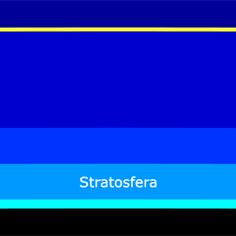
\includegraphics[width=\linewidth]{stratosfera}
		\caption{Položaj stratosfere}
		\label{fig:stratosfera}
	\end{marginfigure} 
Raspodjela temperature u stratosferi zavisi od Sunčeve topiote. U njoj se, za razliku od troposfere, ne javljaju vertikalna kretanja ili su, pak, vrlo slabo izražena. Pored toga, nalazi se neznatna količina vodene pare. Na visini između $22-27km$ ponekad mogu da se vide oblaci, koji su verovatno sastavljeni od vrlo sitnih kapljica prehlađene vode. Postanak ovih oblaka tumači se dovođenjem određene količine vodene pare pri povoljnim uslovima (prekid tropopauze) iz troposfere u stratosfera.\\

\textbf{Mezosfera} obuhvata sloj atmosfere od stratosfere pa do visine od oko 80km. Pogranični sloj između stratosfere i mezosfere naziva se stratopauza. Načelno, mezosfera se odlikuje sa dva sloja, i to prvim — toplim, i drugim — hladnim. Topli sloj se rasprostire od stratopauze pa do visine $50-55km$. U njemu temperatura brzo raste sa porastom visine, tako da na visini $ 40-50km$ iznosi prosjecno $0 ^\circ$C, a u pojedinim slučajevima može da bude i preko $+40^\circ$C. 

	\begin{marginfigure}%
		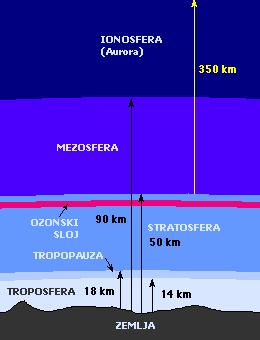
\includegraphics[width=\linewidth]{atmosfera2}
		\caption{Položaj mezosfere}
		\label{fig:atmosfera2}
	\end{marginfigure}
Porast temperature uslovljen je apsorpcijom kratkotalasne Sunčeve radijacije od strane ozona, kao i toplotnim zračenjem Zemlje. U ovom sloju se ne pojavljuju vertikalna kretanja. Iznad visine $50-55k$m temperatura naglo opada i u blizini gornje granice mezosfere dostiže vrijednost od $-70^\circ$C do $ 90^\circ$C. Hladni sloj, za razliku od toplog, karakteriše se turbulencijom i većim brzinama vjetra.\\

\textbf{Termosfera} je sloj atmosfere koji se nalazi iznad mezosfere. U njoj temperatura neprekidno raste sa porastom visine i pretpostavlja se da na visini 200km dostiže vrednost od $200^\circ$C do $250^\circ$C. Prelazni sloj između mezosfere i termosfere naziva se mezopauza. Gornja granica termosfere nalazi se na visini od 800 do 1000km. U termosferi gustina vazduha je vrlo mala. Tako na visini 500km ona u prosjeku iznosi $2.28\cdot10^{-15} g/cm^{3}$  , a na visini od 800km iznosi $6.63\cdot10^{-17} g/cm^{3}$. 

	\begin{marginfigure}%
	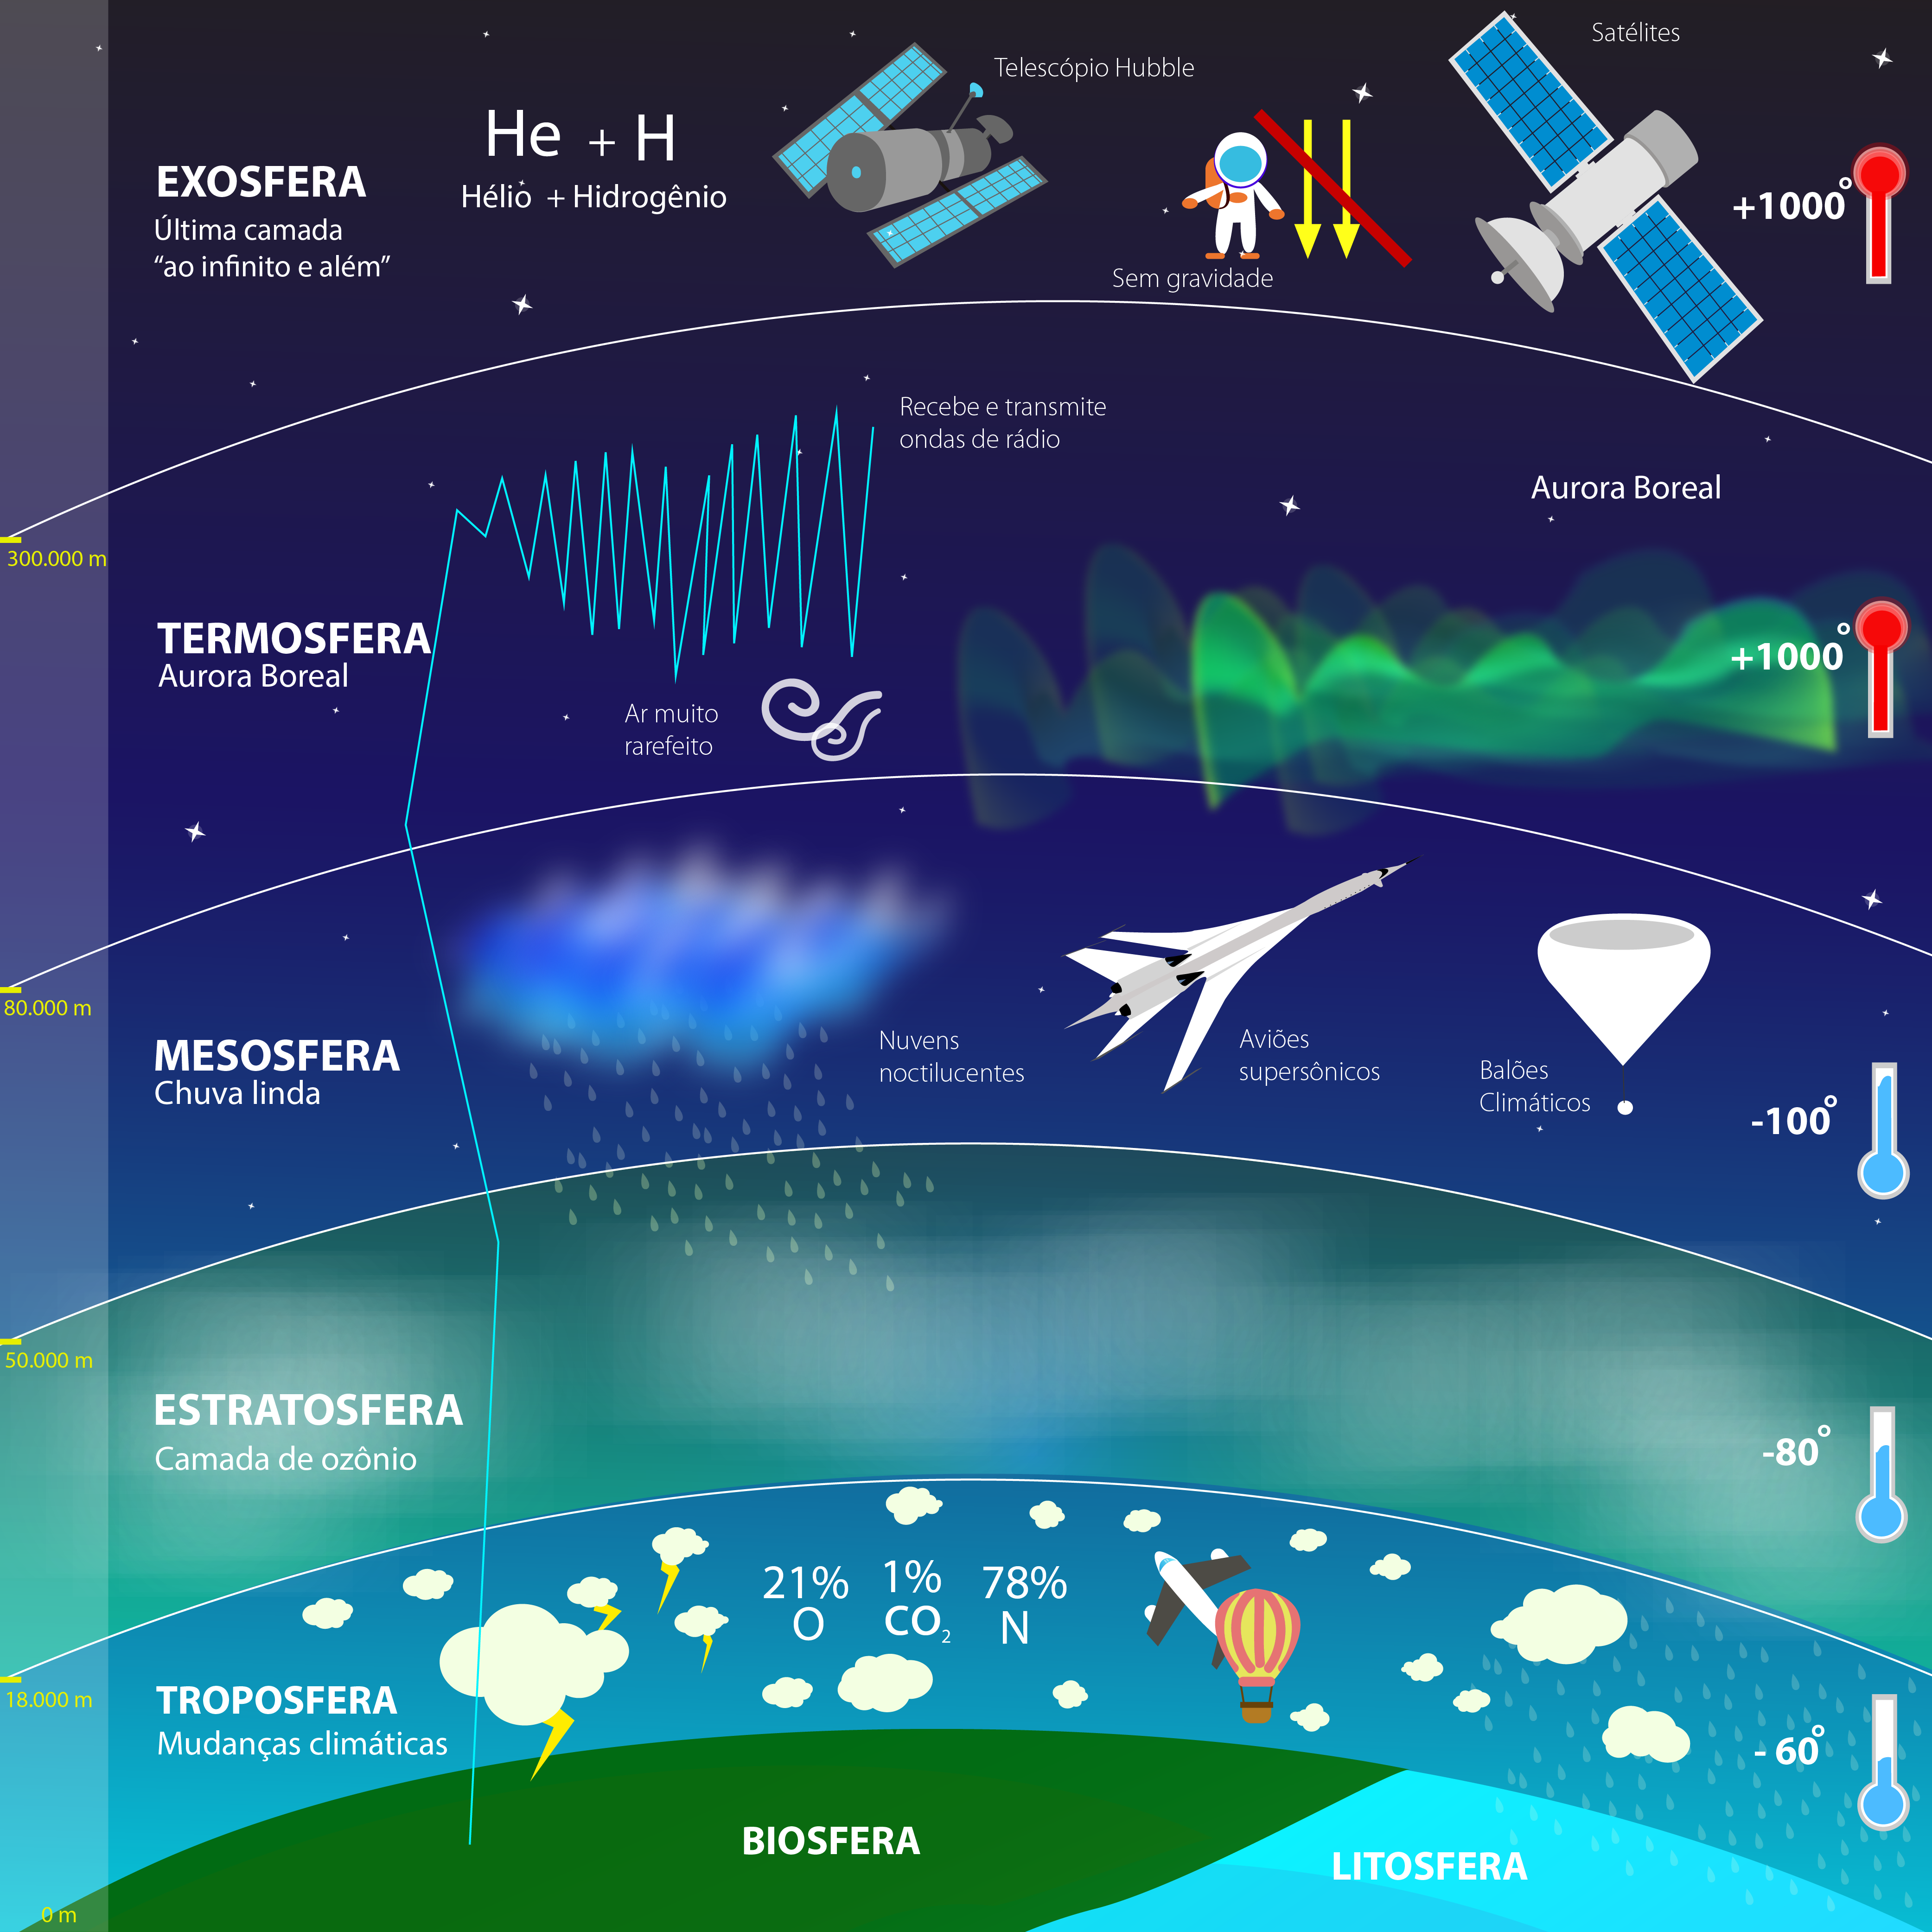
\includegraphics[width=\linewidth]{atmosfera3}
	\caption{Položaj termosfere i egzosfere}
	\label{fig:atmosfera3}
	\end{marginfigure}
Donja polovina termosfere u osnovi se sastoji od ogromnog broja jona, pa se zbog toga i naziva jonosferom. Ovaj se sloj karakteriše vrlo velikom električnom provodljivošću. U poređenju sa vazduhom pri neposrednoj površini Zemlje, električna provodljivost na visini od $100km$ je za nekoliko milijardi puta veća. Ipak, u jonosferi se izdvaja nekoliko slojeva, koji, u odnosu na okolnu sredinu, posjeduju znatno veću koncentraciju jona, a time i veću sposobnost da odbijaju, apsorbuju i prelamaju, u većem ili manjem stepenu, radiotalase. Na broj jona u pojedinim jonosferskim slojevima utiče i Sunčevo ultraljubičasto i X-zračenje. \\

\textbf{Egzosfera} je najviši sloj atmosfere, a rasprostire se od termosfere ka međuplanetarnom prostoru. Između termosfere i egzosfere nalazi se prelazan granični sloj termopauza. Rastojanje između čestica gasa u egzosferi toliko je veliko da pojedine čestice (uglavnom helijuma i vodonika), savlađujući silu Zemljine teže, odlaze u međuplanetarni prostor, i obrnuto  iz međuplanetarnog prostora ulaze u egzosfera.


\section{Sastav i gustina vazduha}

\marginnote[-25pt]{ 
	\subsection{Vazduh} 
	je smjesa, nekih stalnih gasova i ostalih primjesa, koje se tu nalaze u vidu raznih hemijskih jedinjenja te raznih čvrstih, tečnih i gasovitih tvari.\\
}

Glavni sastojci atmosfere su: azot, kiseonik, inertni gasovi i ugljendioksid, ne računajući primjese, koje se gotovo redovno javljaju samo u tragovima. Od primjesa spomenućemo samo neke naj glavni je kao: amonijak, azotni oksidi, jedinjenja sumpora, hloridi, prašina, vodena para, razni mikroorganizmi itd.
Srazmjera glavnih sastojaka vazduha je dosta postojana, pa možemo reći da ona vrijedi za cijelu troposferu.

	\begin{margintable}[0pt]\index{typefaces!sizes}
		\footnotesize%
		\begin{center}
			\begin{tabular}{lc}
				\toprule
				Gas & Procenat $ \% $ \\
				\midrule
				Azot     & $78.03$  \\
				Kiseonik      & $20.99$  \\
				Inertni gasovi     & $0.95$  \\
				Ugljen dioksid    & $0.03$  \\
			
				\bottomrule
			\end{tabular}
		\end{center}
		\caption{Procentualni sastav najvažnijih vazdušnih sastojaka}
		\label{tab:sastav-atm}
	\end{margintable}

	\marginnote[5pt]{ 
		Iz tabele se jasno vidi da su glavni sastojci atmosfere u stvari azot i kisik i da oni zauzimaju više od $99\%$ cijele zapremine.
	}

Poseban značaj među dodacima suhom vazduhu ima vodene para. Ona učestvuje vrlo aktivno u mnogim vremenskim procesima, a pored toga ona znatno slabi Sunčevo zračenje i izračivanje toplote od strane Zemlje. Njezina količina u atmosferi je veoma promjenljiva, a u atmosferi se može pojaviti u sva tri agregatna stanja. U nižim slojevima atmosfere ona može pri toplom i vlažnom vremenu dostići i do $4\%$ zapremine, a u toku jako hladnih zimskih dana ona može da spadne i do blizu $0\%$.

Gustina vazduha (masa u jedinici zapremine) zavisi od vazdušnog pritiska i temperature vazduha, a može se odrediti iz jednačine gasnog stanja: 
$$ pV = nRT $$
	\marginnote[0pt]{
		\begin{itemize}
			\item $p$ (pritisak)
			\item $V$ (specifična zapremina)
			\item $R$ (univerzalna gasna konstanta koja za suhi vazdug iznosi $29.27$)
			\item $T$ (temperatura)
		\end{itemize}
	}

Ako gustinu vazduha označimo sa $ \rho_v $, onda zamijenivši u specifičnoj zapremini $ V = \frac{1}{\rho_v}
$, dobivamo da je: 
$$ \rho_v = \frac{p}{RT} $$
Ova jednačina nam jasno govori da gustina vazduha stoji u upravnom odnosu sa vazdušnim pritiskom, a u obrnutom odnosu sa temperaturom, što znači da gustoća vazduha nije stalna veličina, nego se ona mijenja sa promjenom vazdušnog pritsika i temperature vazduha.\\
	\marginnote[0pt]{
		Ako uzmemo da smo na barometru pročitali pritisak $780mm$, a temperatura vazduha da je $ -13^\circ$C, (odnosno $T = 260K$), onda izlazi da je gustina vazduha $\rho_v=1.395kg/m^{3}$ 
	}

Gornja jednačina vrijedi samo za izračunavanje gustoće suhog vazduha, tj. takvog vazduha u kome uopšte nema nimalo vodene pare. Pošto vazduh uvijek ima stanovite količine vodene pare u sebi, a vodena para je lakša od suhog vazduha.
\section{Atmosferski pritisak}
	\marginnote[0pt]{
		Kako se pritisak definiše silom koja djeluje na jedinicu površine, tako je i vazdušni pritisak definisan težinom kojom vazdušni stub djeluje na jedinicu površine. Drugačije rečeno, \textbf{atmosferski pritisak ili vazdšni jeste pritisak koji vazduh svojom težinom vrši na Zemljinu površinu}.
	}

	\subsection{Pojam i promjena}
	Gaisoviti Zemljin omotač, ili vazduh, je tijelo za koje se, doduše, nije znalo da ima svoju težinu sve do Galileja, koji je $1620.$ godine uspio da to eksperimentalno pokaže. Specifična težina suhog vazduha je $773$ puta manja od specifične težine vode, i jedan kubni centimatr suhog vazduha pod normalnim uslovima (gustina $ \rho =1.29 kg/m^{3} $ , pritisak od  $101325Pa$, temp. od $ 0^\circ$C, geogr. širina $ 45 ^\circ$) mase je $ 1/773 = 0.001293g$, a težine $ G=12.65N $.\\
		\marginnote[0pt]{
		Vazdušni pritisak zavisi od:
		\begin{itemize}
			\item kinetične aktivnosti molekul
			\item temperature vazduha
			\item mase molekula i
			\item gravitacije
		\end{itemize}
		}
	\marginnote[0pt]{
		\subsection{Normalni atmosferski pritisak}
		jeste pritisak vazdušnog stuba temperature $ 0^\circ $C na površinu od $1cm^{2}$, mjeren na nivou mora na $ 45^\circ$ sjeverne geografske širine, a koji uravnotežuje težinu živinog stuba visine ($ h $) od $760mm$.
		$$ p = \rho g h $$
		Ako uzmemo da je $ \rho_{Hg} = 13595.1\frac{kg}{m^{3}}$ i $ g = 9.80665 m/s^{2}$, dobijamo $ p= 101325Pa$.
	}
	Vazdušni ili atmosferski (a često ga naizivamo i barometarski) pritisak se mjeri barometrom, a izražava se u milimetrima visine živinog stuba ($mm Hg$)  koji drži ravnotežu vazdušnog stuba istog presjeka. Prema tome, da bi odredili veličinu barometarskog pritiska na nekom mjestu, dovoljno je da odredimo težinu živinog stuba koji njemu drži ravnotežu. Kretanje molekula vazduha po površini uzrokuje pojavu vazdušnog pritiska, koji djeluje u svim pravcima podjednako.
	Pritisak vazduha na određenu horizontalnu površinu jednak je težini mirnog vazdušnog stuba iznad te površine. ($p=101325Pa$)
		
	Ako se za posmatranu horizontalnu površinu uzme površina od $1cm^{2}$, onda se pritisak vaduha na takvu površinu zove \textbf{atmosferski ili vazdušni pritisak}.
	To znači da je vazdušni pritisak na $1cm^{2}$ Zemljine površine jednak težini vazdušnog stuba čiji je poprečni presjek  $1cm^{2}$, a visina od površine Zemlje do gornje granice atmosfere.
	\subsection{Vertikalna raspodjela vazdušnog pritiska}
	
	\subsection{Horizontalna raspodjela vazdušnog pritiska}
	
	\subsection{Mjerenje atmosferskog pritiska}
	
	
	\section{Izvori atmosferske energije}
